\section{Formation of particle stabilized emulsions}

When two partially miscible fluids are mixed, they phase separate into distinct phases to minimize the thermodynamic penalty associated with interfacial formation. 
To inhibit this phase separation, small-molecule surfactants are conventionally employed. A well-known example of such a material is soap, which facilitates the 
emulsification of dirt into droplets suspended in water through mechanical agitation. Surfactants function by reducing the surface tension between the dispersed 
phase (droplets) and the continuous phase (bulk fluid), thereby lowering the interfacial energy penalty associated with phase formation.

Without the addition of a stabilizer, the dispersed phase will coalescence to reduce the surface area of the interface. To facilitate the stability of small
droplets in the continuous phase, stabilizers such as surfactants, particles or bio-polymers are added. These additives reduce the interfacial energy between
phases characterized through the Pieranski model, $ G_{ads} = \sigma A_{rm} (1 - \cos{\theta_c})^2 $, where $G_{ads}$ represents the free energy reduction upon particle 
adsorption, $\sigma$ is the surface tension between the partially miscible fluids, and $ \theta_c $ is the contact angle of the particle. Surfactants and bio-polymers work
through reducing the surface tension between the dispersed and continuous phase. Particle stabilizers work to stabilize emulsions through reducing the interfacial area between
fluids. 

Following their initial discovery, interest in particle-stabilized emulsions waned for several decades. However, since the 1980s, renewed attention has emerged due to 
their applications in food science. A notable example is the stabilization of water droplets in oil by fat crystals, a process used in margarine production. Particle 
stabilization has also gained interest due to its lower toxicity and the potential for sustainable sourcing, particularly through the use of cellulose or chitin 
particles \cite{fujisawa_nanocellulose-stabilized_2017, tang_stimuli-responsive_2016, kalliola_carboxymethyl_2018}. Moreover, conventional chemical surfactants pose 
environmental concerns, as they can be toxic to aquatic life, acting as xeno-hormones and disrupting reproductive processes 
\cite{kaczerewska_environmental_2020, lechuga_acute_2016}.

Compared to surfactant-stabilized emulsions, particle-stabilized emulsions exhibit greater resistance to coarsening, leading to renewed interest in their applications. 
The microstructural properties of these emulsions were extensively studied in the early 2000s by Binks and Lumsdon when they investigated the effect of particle size
on the resulting Pickering emulsion droplet size. \cite{binks_pickering_2001} Their findings 
indicated that the emulsion droplet radius follows the relationship $R_e \propto \frac{\phi_w}{\phi_p}$, where $\phi_w$ and $\phi_p$ represent the volume fractions of water and particles, 
respectively \cite{binks_pickering_2001}. Additionally, they identified several factors influencing the microstructure of Pickering emulsions, including fluid concentration 
and particle wettability. Neutrally wetting particles do not impose a preferential curvature on the interface, whereas non-neutrally wetting particles can lead to the 
formation of bridged droplets, capillary aggregates, and other non-spherical microstructures, shown in Figure \ref{fig:state_diagram_particle_emulsions}

\begin{figure}
    \centering
    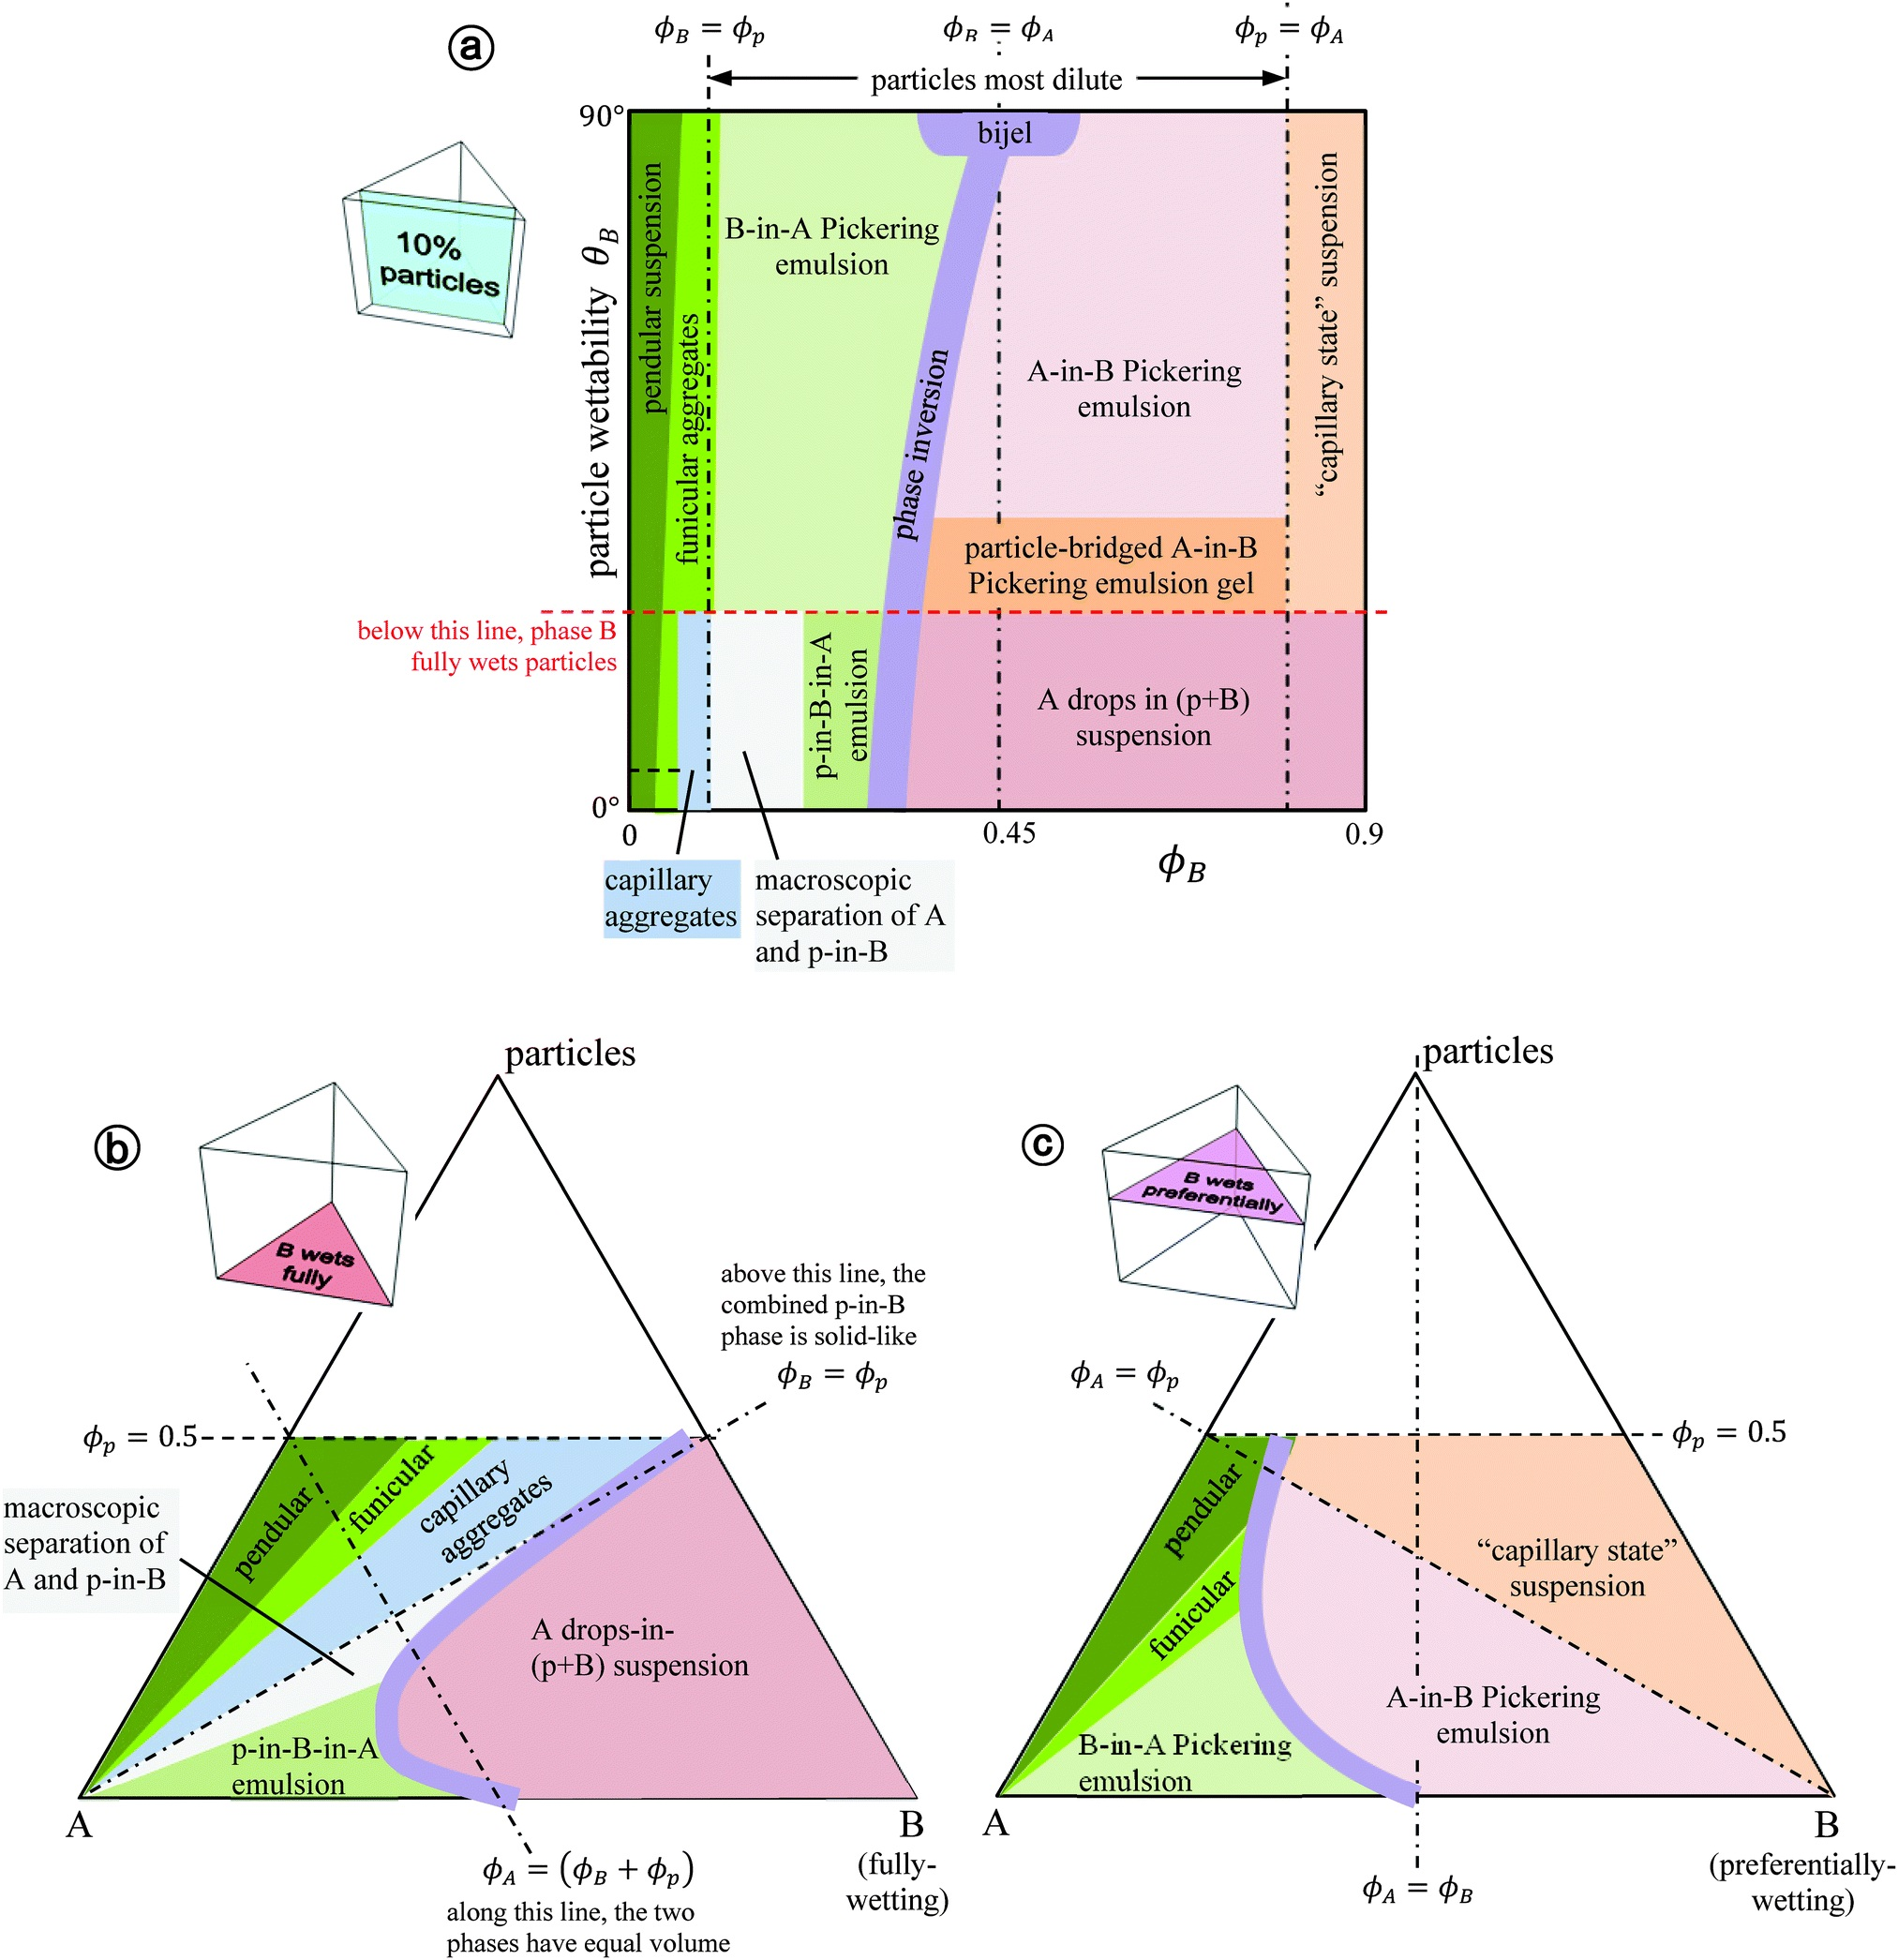
\includegraphics[scale = 0.3]{figures/literature_review/state_diagram.jpg}
    \caption{Formation criteria for a particle stabilized emulsion that can form bijel. \cite{velankar_non-equilibrium_2015}
            Used with permission of Royal Society of Chemistry, from A non-equilibrium state diagram for liquid/fluid/particle 
            mixtures, Velankar, 1, 11, 2015. Permission conveyed through Copyright Clearance Center, Inc}
    \label{fig:state_diagram_particle_emulsions}
\end{figure}

\section{Bicontinuous interfacially jammed emulsion gels}

From Figure \ref{fig:state_diagram_particle_emulsions}, the formation of bijels is shown to require equal volume fraction of fluids and neutrally wetting particles. This
microstructure was first identified in 2005 when Stratford et al. used a multicomponent Lattice Boltzmann Method coupled with particles to characterize the microstructure
and dynamics of particles stabilized emulsions made with equal volume fractions of a binary fluid and suspended particles. \cite{stratford_colloidal_2005} They characterized
that upon initiation of the simulation, the fluids began to undergo spinodal decomposition. As the interface coarsens, particles adsorb onto it. When the particle surface area
and cross sectional area of the particles match, coarsening jams in place resulting in a tortuous co-continuous morphology. A visualization of this process is shown in 
Figure \ref{fig:bijel_coarsen}.

\begin{figure}
    \centering
    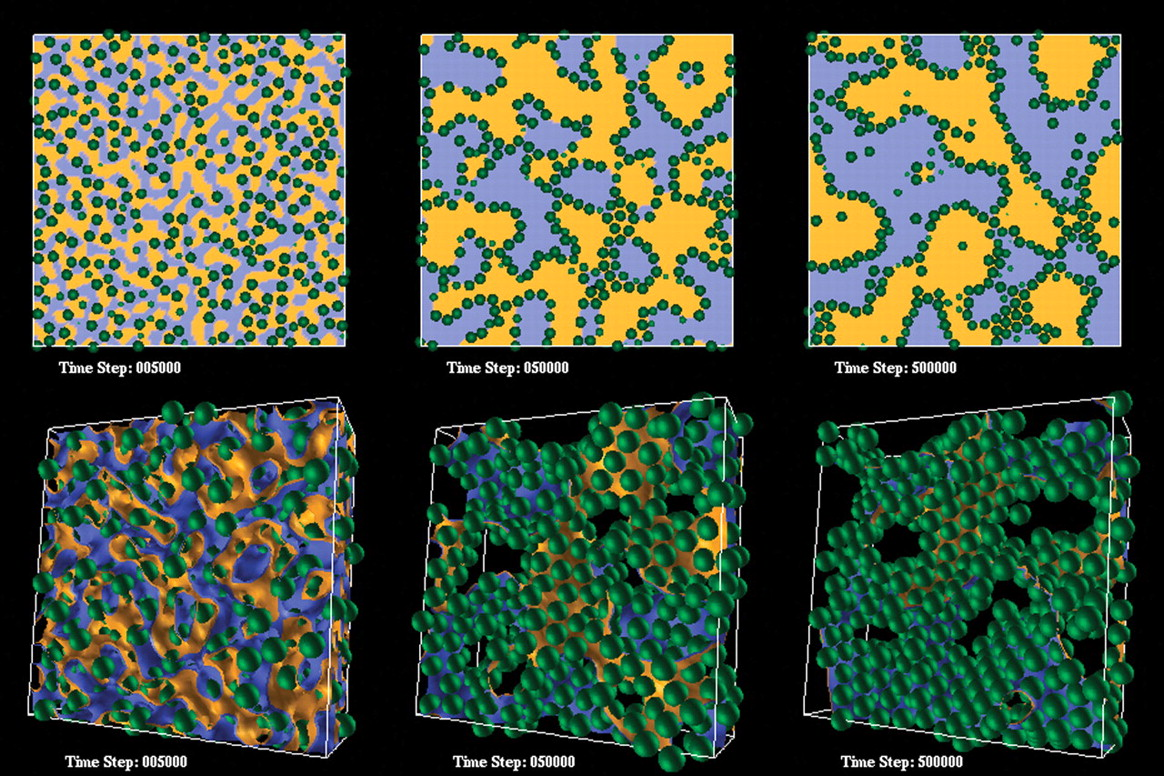
\includegraphics[scale = 0.3]{figures/introduction/bijel_coarsening.jpg}
    \caption{Initiation and arrest of spinodal decomposition as particles adsorb onto the interface, followed by jamming once the 
    interfacial area matches the cross sectional area of the adsorbed particles\cite{stratford_colloidal_2005}. 
    Reproduced from K. Stratford et al., Science 309, 2198-2201(2005) under license number 5966820525314.}
    \label{fig:bijel_coarsen}
\end{figure}

After their discovery in 2005, bijels were realized in experiments in 2007 using a 2-6 lutidine/water system stabilized by surface modified silica particles.
\cite{herzig_bicontinuous_2007} The 2-6 lutidine/water system has a lower critical solution temperature (LCST) of 34.1$^{\circ}C$ and a critical weight fraction of
approximately 28 \% lutidine. \cite{herzig_bicontinuous_2007} Herzig et al. began with a fluid mixture at the critical weight fraction and raised the 
temperature past the LCST, initiating phase separation. \cite{herzig_bicontinuous_2007} This process is known as Thermally Induced Phase Separation (TIPS). 
The domains of the fluid coarsened until they observed
gelation of the system. \cite{herzig_bicontinuous_2007} Since then, other systems based on small molecules, oligomers and polymers have been prepared. 
\cite{tavacoli_novel_2011, lee_bicontinuous_2010, bai_dynamics_2015, ching_rapid_2021} These works have been primarily based on
thermally induced phase separation although as this literature review will show modern bijel fabrication techniques have moved
away from this method to induce phase separation.

Computational simulations have investigated the effect of fluid density, surface tension and particle volume fraction.
\cite{jansen_bijels_2011} Jansen and Harting utilized a multicomponent Lattice Boltzmann method to assess the effect of fluid volume fraction,
particle volume fraction, surface tension, fluid density and particle contact angle on the microstructure of particle stabilized emulsions.
They demonstrated that the effect of the surface tension and initial fluid density were small
compared to the volume fraction of particles by measuring the length scale of the bijels. \cite{jansen_bijels_2011} The length of 
particles was proportional to the inverse of the particle volume fraction, $L \propto \frac{1}{\phi_p}$. \cite{jansen_bijels_2011} 
Jansen and Harting also illustrated that the emulsion state obtained, whether a Pickering emulsion or bijel, was most affected by 
the contact angle of the particle stabilizer and fluid ratio rather than the particle volume fraction. \cite{jansen_bijels_2011}

Further investigations of the bijel microstructure look at calculating the morphology of the bijel through topological, geometric 
or image analysis techniques. Topological techniques include the quantification of the genus and channel size distribution which
allow for determination of differences in the interfacial properties. \cite{chan_channel_2012} Chan and Thornton compared the topology
of bicontinuous systems obtained using the Cahn-Hilliard and Allen-Cahn equations and identified how they differed. \cite{chan_channel_2012}
Topological techniques have the advantage
of being able to characterize the microstructure of a bicontinuous material while also providing information about the connectivity of the
structure. 

Geometric techniques such as
calculating the curvature of the bijel have also been used to identify the impact of particle size and quench rate on the microstructure
of bijels. Reeves et al. compared the Gaussian curvatures of bijels stabilized with micro and nanoparticles, as well as the effect of quench rate
on bijels formed using thermally induced phase separation to characterize that reduced particle size resulted in the interface maintaining a more negative
Gaussian curvature. \cite{reeves_particle-size_2015,reeves_quantitative_2016}
The interface of bijels are most similar to minimal surfaces, which indicates their mean curvature and Gaussian curvature are 0 and negative respectively. 
\cite{jinnai_interfacial_2001} Nanoparticles are able to conform to curved surfaces better as they are less disruptive to the curvature of the interface, resulting
in more effective stabilization of saddle like regions. \cite{reeves_quantitative_2016} 

Image analysis techniques have also been used to characterize the microstructure of bijels, providing information on the connectivity, pore size
distribution, tortuosity and self similarity. \cite{mcdevitt_microstructural_2019,reeves_quantitative_2016} Connectivity can be derived from region
growing algorithms, labelling algorithms such as Hoshen-Kopelmann and segmentation. \cite{mcdevitt_microstructural_2019,reeves_quantitative_2016}
The pore size distribution can be obtained from watershed algorithm. \cite{mcdevitt_microstructural_2019}

\section{Bijel synthesis techniques}

TIPS has enabled batch synthesis of bijels in research laboratories. However, for bijels to become industrially viable, a continuous fabrication process is required.
This technique should also be flexible enough to produce tailored bijel microstructures to different applications. Solvent Transfer Induced Phase Separation (STrIPS) 
has been shown as a method to achieve this, shown in Figure \ref{fig:strips}. Figure \ref{fig:strips}a) shows the preparation of casting mixture in STrIPS. The casting
mixture is a ternary fluid system comprised of the fluids making up the bijel and a solvent. Figure \ref{fig:strips}b) demonstrates the removal of solvent from the
casting mixture, by flowing a co-solvent past the casting mixture, initiating phase separation. A narrow range of compositions can be used to ensure that the composition
of the phase separating mixture remains within the spinodal line of the demixed region of the phase diagram. Figure \ref{fig:strips} shows how varying the flow rate
of the casting mixture and the solvent removal medium is necessary to control the morphology of the bijel. 

\begin{figure}[h]
    \centering
    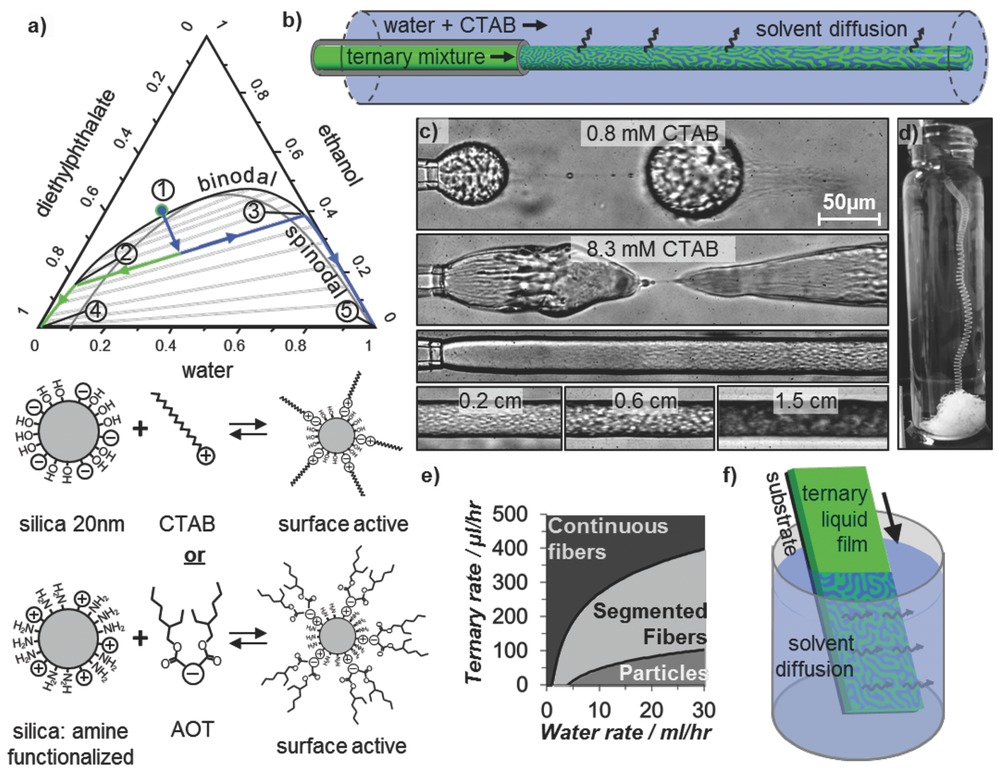
\includegraphics[scale = 5]{figures/introduction/STrIPS.jpg}
    \caption{STrIPS in action. Extrusion of the bijel casting mixture into a non-solvent bath, followed by removal of solvent from 
             the casting mixture through diffusion. \cite{haase_continuous_2015}. Reproduced with permission from Wiley-VCH Verlag GmbH 
             \& Co. KGaA from \textit{Continuous Fabrication of Hierarchical and Asymmetric Bijel Microparticles, Fibers, and Membranes by 
             Solvent Transfer-Induced Phase Separation (STRIPS)}, Haase, M. F., Stebe, K. J., 
             \& Lee, D., \textit{Advanced Materials}, 27(44), 7065-7071, 2015}
    \label{fig:strips}
\end{figure}

STrIPS has been used extensively in a variety of systems ranging from bijels for battery electrode templates, to drug delivery medium, liquid in liquid printing and
intrinsically polymerizable bijels facilitating the production of free standing structures.
\cite{garcia_scalable_2019,thorson_bijel-templated_2019, amirfattahi_fabrication_2024, ching_rapid_2021} STrIPS is flexible to the casting mixture being used. The
only requirement a casting mixture used for STrIPS is that the phase diagram for the casting mixture must be well understood so that the solvent transfer step remains
within the spinodal at all times. 

Another technique based on the removal of solvent is Vapor Induced Phase Separation(VIPS). \cite{wang_scalable_2020} A quarternary casting mixture
containing particles, solvent and two partially miscible liquids is prepared. The solvent and liquid species and compositions are carefully selected to ensure that 
removal of the solvent will cause phase separation of the two partially miscible liquids through the critical point of the phase diagram. This ensures that phase separation
only occurs through spinodal decomposition. One system that has been 
used is the water/hexanediol-diacrylate solvated by ethanol. Removal of ethanol at room temperature is sufficient to facilitate bijel formation, with this bijel
mixture composition being able to be spray or blade coated. This technique is limited by the temperature dependence of surface tension, meaning that the casting mixtures
that can be used are limited to solvents that can vaporize at room temperature.

Instead of relying upon spinodal decomposition to generate the bijel morphology, homogenization uses shear to join phase separating domains, resulting in a 
structure that has the properties of a bijel even if not fabricated from fluids undergoing spinodal decomposition. \cite{huang_bicontinuous_2017, cai_bijels_2017} 
This method is primarily used for nanoparticles under $50$ nm and it has been shown to work for multiple particle geometries. This method relies upon
shear to cause limited coalescence of droplets. As coarsening occurs, particles adsorb on the interface and when the interfacial area matches the area of the
adsorbed particles, the microstructure jams. Microstructure tuning of the method can be done through modifying the contact angle of the particles through addition of
surfactants or viscosity of the phase separating fluids through the addition of viscosity modified such as oligomers. Thus far, all these synthesis techniques use
spherical particles to stabilize the bijels that are generated. 

\section{Ellipsoidal particles at interfaces}

Over the past decade, advancements in synthesis techniques have significantly expanded the ability to fabricate particles with anisotropic geometry and surface chemistry. 
The choice of synthesis method depends on the desired particle shape. For example, ellipsoidal particles can be readily produced through the mechanical deformation of 
polymer spheres, while dumbbell-shaped particles can be synthesized using microfluidic devices or emulsion templating. \cite{fei_magneto-capillary_2020} 
Square-shaped particles, on the other hand, can be 
generated through controlled crystallization \cite{morgan_understanding_2013}. The increasing variety of synthesis methods has reduced geometric constraints when exploring 
potential particle stabilizers for bijels \cite{wu_recent_2016}.

\begin{figure}
    \centering
    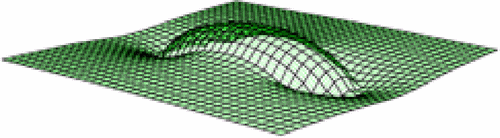
\includegraphics[scale = 0.5]{figures/literature_review/interfacial_curvature.png}
    \caption{Quadropolar capillary interactions around prolate ellipsoidal particles caused by interfacial deformations 
             around the particle. \cite{loudet_capillary_2005} Reprinted Figure 4 with permission from
             Loudet et al, Phys. Rev. Letter., 94, 08301, 2003 Copyright 2025 by the American Physical Society.}
    \label{fig:anisotropic_particle_interface}
\end{figure}

Anisotropic particles exhibit shape-dependent properties due to their ability to induce multipolar interactions by deforming the interface to maintain a mean curvature of 
zero, thereby satisfying the Young-Laplace equation, as illustrated in Figure \ref{fig:anisotropic_particle_interface} \cite{loudet_capillary_2005, cheng_shape-anisotropic_2013}.
This property has been leveraged to facilitate directed assembly and migration through modified capillary forces imparted through curvature gradients at interfaces.
\cite{cavallaro_curvature-driven_2011, read_dimerization_2020, sharifi-mood_curvature_2015}. Simulations have shown that ellipsoidal particles can adopt metastable orientations depending upon the perturbations 
the particle experiences. \cite{gunther_lattice_2013}
% The adsorption process is affected by the shape of particles used as they pack differently onto the interface \cite{hijnen_bijels_2015, daware_emulsions_2015,carmack_diverse_2017}. It has also been suggested that adsorption dynamics of ellipsoidal particles at liquid interfaces are driven completely by viscous forces even if the timescales of adsorption are driven by particle properties \cite{Coertjens2017}. Some guiding equations to calculate the interfacial area of an ellipsoidal particle are provided \cite{gunther_timescales_2014, Davies2014}.

Ellipsoidal particles have been used as stabilizers in bijels, resulting in bijels that have smaller domains than those made with spherical particles
at the same volume fraction, identified to arise from the  greater surface area to volume ratio of ellipsoidal particles compared to spherical particles. 
\cite{gunther_timescales_2014} The evolution of the microstructure is also distinct to bijels stabilized with spheres, demonstrating two timescales at
early and later timesteps. \cite{gunther_timescales_2014} The short timescale is during formation of the bijel, when particles are adsorbed onto the
interface and rotate to align with the interface. At longer timescales, capillary interactions between particles lead to reordering of particles
at the interface, leading to a different interfacial configuration and microstructure. \cite{gunther_timescales_2014}

Rod like particles have also been used as stabilizers in experiments, identifying that the length scale of the pores of 
the bijels follows $ L \propto \frac{1}{\phi_p} $ even if the proportionality constant is different. While the proportionality constant depends on 
particle geometry, this trend has been observed across various particle shapes 
\cite{hijnen_bijels_2015, madivala_exploiting_2009, gunther_timescales_2014, daware_emulsions_2015, loudet_capillary_2005, cheng_shape-anisotropic_2013}.
The dynamics of bijels stabilized by ellipsoidal particles are also distinct from bijels stabilized by spheres, caused by reorientation of particle
stabilizers at the interface. 

\section{Magnetic fields applied to particles at interfaces}

Magnetic fields offer a non-invasive and targeted method for manipulating the behavior of particles. Magnetic particles can be fabricated from
coatings applied onto particles through deposition techniques or a core-shell particle that encapsulates a magnetic core with a non-magnetic shell. 
\cite{fei_magneto-capillary_2020, nakayama_stimuli-responsive_2018} These effects arise due to the interplay between the magnetic torque or force 
acting on the particles and the capillary interactions that govern their behavior at the interface. One theory developed for neutrally wetting ellipsoidal 
particles is Bresme-Faraudo theory. \cite{bresme_orientational_2007, davies_interface_2014}

A wide range of behaviors has been observed when magnetic fields are applied to interfacial particles. Individual particles tend to align their magnetic 
dipole moments along the direction of the field, causing them to reorient relative to the interface. \cite{kim_bijels_2010}
For anisotropic particles such as ellipsoids, this results in a tilt or rotation that changes their interfacial footprint and local curvature. 
\cite{davies_assembling_2014, davies_interface_2014} The orientation of the particle is a function of the capillary interactions with the interface that 
prefers to keep the particle flat on the interface and the magnetic field that is attempting to rotate the particle out of the interface. The magnetic force
experienced by the particle is a function of the applied field strength, magnetic susceptibility, size of the particle, shape of the particles 
and aspect ratio of the particle. 

The equilibrium and metastable orientations of non-spherical particles at fluid interfaces are governed by a complex interplay of particle shape, 
interfacial tension, and external forces such as magnetic fields. Depending upon the surface wettability and aspect ratio of the particle, non-spherical
particles have been observed to adopt several stable and metastable orientations. \cite{morgan_understanding_2013, newton_influence_2014}

Studies on superellipsoidal hematite particles have demonstrated that isolated 
anisotropic particles at the oil–water interface can adopt multiple stable and metastable orientations depending on their aspect ratio and surface 
wettability. Specifically, particles exhibit orientations where their major or minor axes align either parallel or perpendicular to the interface, 
with each configuration corresponding to a local or global energy minimum depending on the interfacial energy landscape \cite{1}. Lattice Boltzmann 
simulations further support these findings, revealing that particle aspect ratio significantly influences the contact angle and immersion depth, 
which in turn affect the energetic favorability of different orientations \cite{3}. In the presence of a magnetic field, these equilibrium states can 
shift due to the torque exerted on the particles, aligning their magnetic moments with the field direction. Experimental observations confirm that 
magnetic anisotropic particles, such as hematite ellipsoids, can be reoriented at the interface by applying a magnetic field, leading to controlled 
transitions between metastable and stable states \cite{2}. These studies collectively show that the equilibrium orientation of anisotropic particles 
is not singular, but rather a function of particle geometry, field strength, and interfacial anchoring, with metastable states playing a significant 
role in the dynamic reconfiguration of interfacial structures.

In many particle system, the magnetic field driven interfacial reorientation lead to the formation of linear chains or clusters of particles on flat interfaces. 
\cite{davies_assembling_2014, davies_interface_2014,newton_influence_2014, newton_capillary_2018} The orientation of particles relative to one another is also
a function of the number of particles in contact and the applied field strength owing to the magnetic field driven interactions between each particle. 
\cite{newton_influence_2014, newton_capillary_2018} In Pickering emulsions, this has enabled field-controlled droplet deformation, coalescence, 
and motility, illustrating the potential for on-demand manipulation of interfacial structures. \cite{melle_pickering_2005, tham_magnetophoresis_2021} 

\textcolor{blue}{stuff about how magnetic fields affect rheology in pickering emulsions}



\section{Rheological models and shear response of particle stabilized emulsions}

Bijels undergoing constant shear demonstrate shear thinning behavior which at moderate shear rates can be described reasonably well using the Herschel-Buckley
model. \cite{macmillan_rheological_2019, wang_morphology_2023} At higher shear rates, the bijel microstructure is destroyed and the viscosity becomes newtonian. 
\cite{cai_bijels_2017,bonaccorso_shear_2020}. Figure \ref{fig:bijel_under_shear} illustrates the findings of Bonnacorso et al., which observed that when a bijel 
stabilized with hard-sphere-like particles is subjected to shear, the particles initially align with the shear direction before detaching from the interface 
\cite{bonaccorso_shear_2020}. Investigating the impact of particle alignment on rheology, prior studies in suspension rheology have shown that colloidal systems 
with hard-sphere interparticle interactions undergoing constant shear exhibit shear banding—where particles order in the shear direction at moderate shear rates—resulting 
in shear thinning \cite{vermant_flow-induced_2005, brader_nonlinear_2010}. 

\begin{figure}
    \centering
    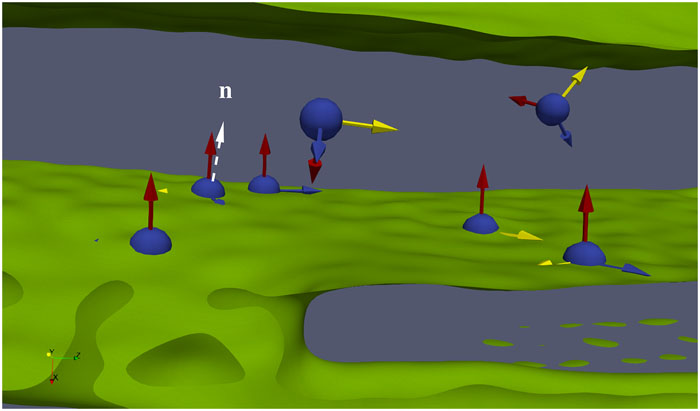
\includegraphics[scale = 3]{figures/literature_review/bijel_under_shear.jpeg}
    \caption{Schematic of a bijel with hard-sphere particles undergoing shear, demonstrating migration and detachment of 
             particles at the interface. \cite{bonaccorso_shear_2020} Reproduced from Shear dynamics of confined bijels
             ,Bonaccorso et al. AIP Advances 1, September 2020; 10 (9): 095304, under the Creative Commons CC BY License.}
    \label{fig:bijel_under_shear}
\end{figure} 

Studies on complex bijel rheology have demonstrated gel-like characteristics when the storage modulus exceeds the loss modulus \cite{lee_making_2013, bai_dynamics_2015}. 
Ching and Mohraz further showed that the rheological behavior of bijels closely resembles that of a 2D colloidal glass percolating in 3D space, based on comparisons of 
linear viscoelasticity with colloidal gels composed of strongly attractive particles \cite{ching_bijel_2022}. Key characteristics of glasses include the presence of a 
yield stress, viscoelastic behavior, and a glass transition point \cite{pham_yielding_2008, weeks_introduction_2017}. Yield stress corresponds to the applied stress at 
which the particle monolayer undergoes irreversible structural changes \cite{pham_yielding_2008}. Viscoelasticity arises when the monolayer exhibits both solid and 
liquid-like behavior, depending on the timescale of the applied stress \cite{pham_yielding_2008}. The glass transition point is marked by a dramatic slowdown in the 
monolayer's dynamics \cite{weeks_introduction_2017}. 

Ellipsoidal particles influence the rheological properties and stability of Pickering emulsions. When investigating the effect of rod-like particles on the
rheology of emulsion droplets, Madivala et al. showed that droplets stability under shear increased as the aspect ratio of the rod-like particle increased.
\cite{madivala_exploiting_2009} This was attributed to the more effective interfacial coverage of particles and interface deformations inducing attractive
capillary interactions between particles, reinforcing the particle monolayer to applied shear. \cite{madivala_exploiting_2009} Investigations into the rheology of
Pickering droplets stabilized by graphene nanosheets showed that the dicsc like particles had posessed increased viscosity and viscoelasticity compared to the same 
system synthesized with spherical particles. \cite{imperiali_simple_2014} The elasticity of the interface has been shown to be a function of the particle stabilizer
used. \cite{sun_assembly_2013}

Magnetically responsive Pickering emulsions exhibit rheological behavior that can be tuned by external magnetic fields, making them attractive for applications 
requiring on-demand flow control and structural reconfiguration. \cite{qiao_magnetorheological_2012, melle_pickering_2005} Upon application of a field, particles
order at the interface. This tunable rheology enables reversible transitions between fluid and gel-like states, which is particularly valuable in 
applications such as enhanced oil recovery, drug delivery, and soft robotics \cite{tham_magnetophoresis_2021}.

% \textcolor{blue}{https://www.mdpi.com/2311-5521/5/3/150}

% \section{Colloidal glasses}

% \begin{itemize}
%     \item https://pubs.acs.org/doi/10.1021/acsmacrolett.6b00826
%     \item Add stuff on dynamic heterogeneity
%     \begin{itemize}
%         \item https://pubs.rsc.org/en/content/articlelanding/2012/sm/c2sm25267h
%     \end{itemize}
%     \item Add stuff on particle jamming
%     \begin{itemize}
%         \item https://journals.aps.org/rmp/pdf/10.1103/RevModPhys.82.2633
%     \end{itemize}
%     \item Add stuff on cooperatively rearranging regions
%         \begin{itemize}
%             \item https://doi.org/10.1038/ncomms4829
%             \item https://journals.aps.org/prl/abstract/10.1103/PhysRevLett.110.188301
%             \item https://journals.aps.org/prl/abstract/10.1103/PhysRevLett.107.065702
%         \end{itemize}
%     \item Add stuff on reentrant glass phenomena 
%     \begin{itemize}
%         \item https://doi.org/10.1209/0295-5075/86/58001
%     \end{itemize}
% \end{itemize}

\section{Stimuli response in bijels}

Kim et al. used a free energy based lattice boltzmann method coupled with particles and magnetic fields to investigate the influence of magnetic fields on 
the microstructure of bijels stabilized with spherical particles. \cite{kim_bijels_2010}
They observed that applying strong magnetic fields did not significantly alter the bijel microstructure, as the particles aligned with 
the field without disrupting the interfacial ordering. This finding suggests that spherical particles, due to their isotropic shape, do 
not induce anisotropic stresses on the interface when subjected to magnetic fields, thereby maintaining the structural integrity of the bijel.

In contrast to the minimal impact of magnetic fields on bijels stabilized with spherical particles, Carmack and Millett investigated the effects of 
applied electric fields on thin-film bijels using a Cahn-Hilliard coupled with Langevin dynamics computational model. \cite{carmack_tuning_2018} 
Their study revealed that electric fields can induce significant microstructural changes in bijels, with particles self-assembling into chains and forming 
cylindrical domains aligned parallel to the applied field, thereby modifying the overall microstructure. Carmack and Millet observed that the dielectric contrast 
between liquid domains governs liquid domain alignment, and the dielectric contrast between colloidal particles and the liquid matrix induces dipolar particle 
interactions. By changing the dielectric contrast between particle and fluid, different bijel morphologies could be formed. Additionally, particle chains were found to 
act as nucleation sites for phase separation, influencing the resultant morphologies in terms of particle attachment to phase interface regions and average 
channel diameter. 

While not strictly stimuli-responsive, microstructure modifications have been achieved by applying a particle volume fraction gradient during the formation of 
bijels using Thermally Induced Phase Separation (TIPS). \cite{french_bicontinuous_2022} In their study, French et al. allowed particles to partially sediment in the bijel casting mixture
before initiating thermal quenching. The gradient in particle volume fraction along the height of the reaction vessel caused the jamming point of the bijel
to vary along the gradient axis, causing a channel size gradients of up to 2.8\% per millimeter, as measured using confocal microscopy.